\documentclass[t]{beamer}
\usepackage[T1]{fontenc}
\usepackage[utf8]{inputenc}
\usepackage{lmodern}
\usepackage{lmodern}
\usepackage{biblatex} 
\usepackage{amsmath}
\usepackage{amsfonts}
\usepackage{amssymb}
\usepackage{amsthm}
\usepackage{graphicx}
\usepackage{color}
\usepackage{xcolor}
\usepackage{url}
\usepackage{textcomp}
\usepackage{hyperref}
\usepackage{parskip}
\usepackage{svg}
\usepackage{caption}

\usetheme{CambridgeUS}
\AtBeginBibliography{\footnotesize}
\addbibresource{presentation.bib}

\makeatletter
\setbeamertemplate{footline}
{
  \leavevmode%
  \hbox{%
  \begin{beamercolorbox}[wd=.333333\paperwidth,ht=2.25ex,dp=1ex,center]{author in head/foot}%
    \usebeamerfont{author in head/foot}\insertshortauthor%~~\beamer@ifempty{\insertshortinstitute}{}{(\insertshortinstitute)}
  \end{beamercolorbox}%
  \begin{beamercolorbox}[wd=.333333\paperwidth,ht=2.25ex,dp=1ex,center]{title in head/foot}%
    \usebeamerfont{title in head/foot}\insertshorttitle
  \end{beamercolorbox}%
  \begin{beamercolorbox}[wd=.333333\paperwidth,ht=2.25ex,dp=1ex,right]{date in head/foot}%
    \usebeamerfont{date in head/foot}\insertshortdate{}\hspace*{2em}
    \insertframenumber{} / \inserttotalframenumber\hspace*{2ex} 
  \end{beamercolorbox}}%
  \vskip0pt%
}
\makeatother

\title{Knowledge-Based Question Answering}
\author{Sudipto Ghosh}
\institute{\emph{M.Sc. CS Semester I\\Department of Computer Science\\University of Delhi}}
\date{\today}

\begin{document}

\begin{frame}
    \titlepage
\end{frame}

\begin{frame}
    \frametitle{Overview}
    \tableofcontents
\end{frame}

\section{Problem Statement}
\subsection{Problem Definition}
\begin{frame}
    \frametitle{Problem Definition}
    \begin{itemize}
    \item Parse unstructured text from domain corpus, identify entities, extract relations, map relations to domain concepts and build knowledge base.\\
    \textbf{Input:} Corpus, domain ontology, and training examples consisting of entity boundaries, relationship dependencies, valid triples.\\
    \textbf{Output:} <s,p,o> triples to populate the knowledge graph.
    \item Model natural language question into a query, infer the facts about it required for the answer, assemble the facts into a natural language answer, and present it to the user.\\
    \textbf{Input:} Question as a spoken utterance or text prompt.\\
    \textbf{Output:} Answer/fact as a spoken utterance or text response.
    \item Ensure system maximizes performance on giving correct answers to a set  of competency questions. 
    \end{itemize}
\end{frame}

\subsection{Motivation}
\begin{frame}
    \frametitle{Motivation}
    \begin{itemize}
    \item Leveraging domain knowledge to improve virtual assistants.
    \item Inferencing step $\implies$ system can answer unanticipated questions.
    \item Level of detail can be controlled to suit the expertise of the user.
    \item Can we answer complex questions that contain multiple subjects, express compound relations, or require simulated thinking?
    \end{itemize}
    
    \begin{example}
    \textbf{Q:} What is the capital of India?\\
    \textbf{A:} The capital of India is New Delhi.\\
    \textbf{Q:} What is the state of motor 2?\\
    \textbf{A:} Motor 2 is currently turned off.
    \end{example}
\end{frame}

\subsection{Modelling}
\begin{frame}
    \frametitle{Modelling}
    \begin{block}{Information Retrieval Agent}
    Given documents forming the domain corpus $D$, extract facts and construct a knowledge graph containing entities and semantic relations between them. Percepts are continuously made available in light of quick-updating corpus, knowledge in the KG may be revised based on incoming facts.
    \end{block}
    \begin{block}{Conversational KBQA Agent}
    Given a KG built from facts in domain corpus $D$ and a conversation history ($Q_1$, $A_1$, $Q_2$, $A_2$, $\ldots$), the goal for an reading comprehension / knowledge based conversational QA agent is to answer the $n^{th}$ question $Q_n$ using the whole conversation history as context.\\
    However, in an open domain conversational QA, user can switch between topics, making the conversation history irrelevant.
    \end{block}
\end{frame}

\section{Modules}
\subsection{KB Construction}
\begin{frame}
    \frametitle{KB Construction}
    \begin{itemize}
    \small{\item Knowledge base construction (KBC) is the process of populating a knowledge base (KB) with facts (or assertions) extracted from data.}
    \end{itemize}
    \begin{block}{Sentence}
        \scriptsize{Paracetamol, also known as acetaminophen, is usually prescribed for treating fever}
    \end{block}
    \begin{block}{Entity Recognition}
        \scriptsize{{\color{red} Paracetamol}, also known as {\color{red} acetaminophen}, is usually prescribed for treating {\color{red} fever}}
    \end{block}
    \begin{block}{Relation Extraction}
        \scriptsize{{\color{red} Paracetamol}, also {\color{teal} known as} {\color{red} acetaminophen}, is usually {\color{teal} prescribed for} treating {\color{red} fever}}
    \end{block}
    \begin{block}{Coreference Resolution}
        \scriptsize{{\color{red} Paracetamol}, also {\color{teal} known as} {\color{red} acetaminophen} | {\color{red} Paracetamol} is usually {\color{teal} prescribed for} treating {\color{red} fever}}
    \end{block}
\end{frame}

\begin{frame}
    \frametitle{KB Construction (contd.)}
    \begin{block}{Triple Extraction}
        \tiny{<{\color{red} Paracetamol}, {\color{teal} known as}, {\color{red} acetaminophen}>\\ <{\color{red} Paracetamol}, {\color{teal} prescribed for}, {\color{red} fever}>}
    \end{block}
    \begin{block}{Entity Linking}
        \tiny{<{\color{red} https://en.wikipedia.org/wiki/Paracetamol}, {\color{teal} known as}, {\color{red} https://en.wikipedia.org/wiki/Acetaminophen}>\\ <{\color{red} https://en.wikipedia.org/wiki/Paracetamol}, {\color{teal} prescribed for}, {\color{red} https://en.wikipedia.org/wiki/Fever}>}
    \end{block}
    \begin{block}{Ontology Mapping}
        \tiny{prefix {\color{teal} wikidata https://www.wikidata.org/wiki/Property}}\\~\\       \tiny{<{\color{red} https://en.wikipedia.org/wiki/Paracetamol}, {\color{teal} wikidata:P2561}, {\color{red} https://en.wikipedia.org/wiki/Acetaminophen}>\\ <{\color{red} https://en.wikipedia.org/wiki/Paracetamol}, {\color{teal} wikidata:P2176}, {\color{red} https://en.wikipedia.org/wiki/Fever}>}
    \end{block}
    \begin{itemize}
    \small{\item The resultant triples are stored to a triple or RDF store like Blazegraph through semantic queries, or a graph database like Neo4J.}
    \end{itemize}
\end{frame}

\begin{frame}[c]
    \begin{figure}[h]
    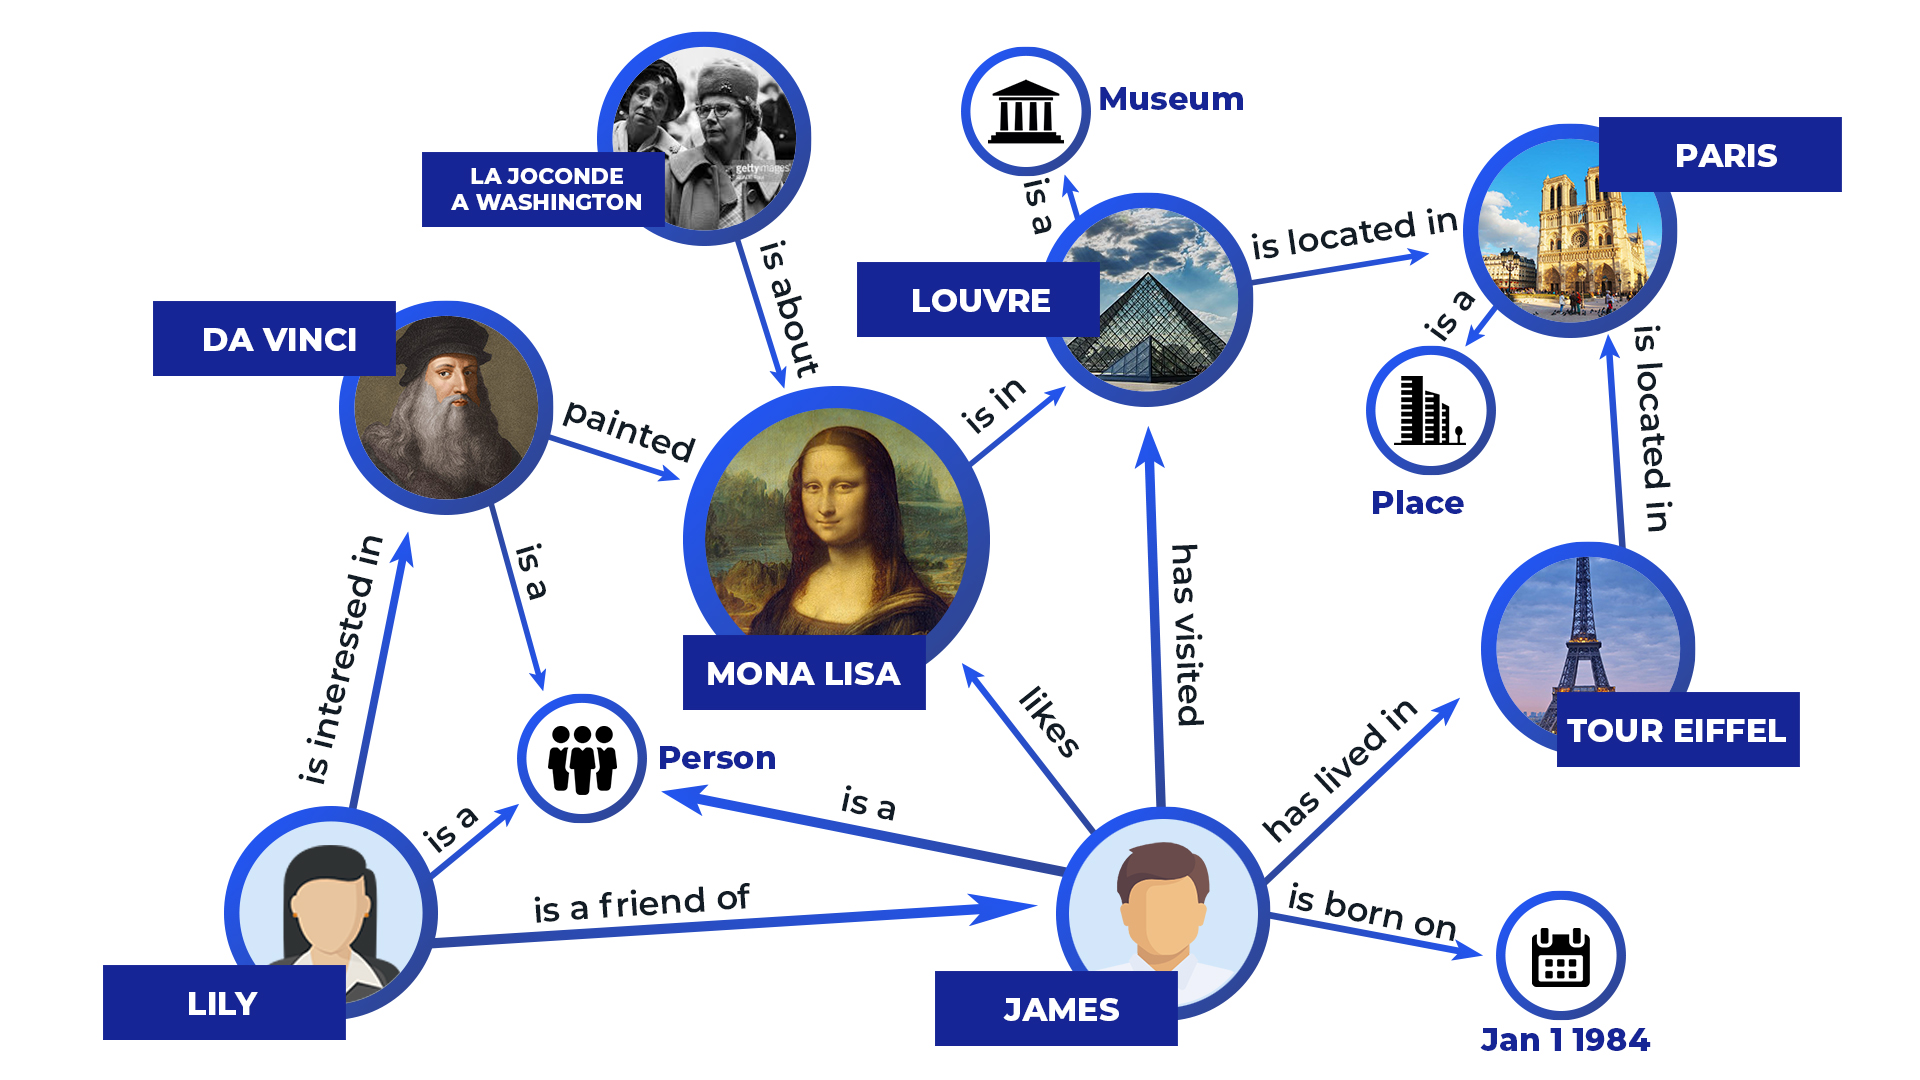
\includegraphics[width=120mm]{knowledge-graph-example.jpg}
    {\caption*{\tiny{\emph{Source: Let The Machines Learn}}}}
    \end{figure}
\end{frame}

\begin{frame}
    \frametitle{How?}
    \begin{itemize}
        \item Data Collection - scrape domain repository, select domain ontology.
        \item Use rule-based approaches (e.g. JAPE Grammar) to gather facts from the documents?
        \item Use language models (e.g. BERT, RoBERTa) and fine-tune it to do the fact extraction?
        \item Representation Format - RDF, Turtle, N3 in Triple Store - KG.
        \item Entity Linker needs a KG/Linked Open Data to map entities to.
    \end{itemize}\
    \begin{block}{Turtle - Terse RDF Triple Language}
        \small{RDF Graph in a compact, textual form.}\\
        {\tiny <http://example.org/\#spiderman> <http://www.perceive.net/relationship/enemyOf> <http://example.org/\#green-goblin> .
        <http://example.org/\#spiderman> <http://xmlns.com/foaf/0.1/name> "Spiderman" .}
    \end{block}
\end{frame}

\begin{frame}[c]
    \centering JAPE Grammar\\
    \centering 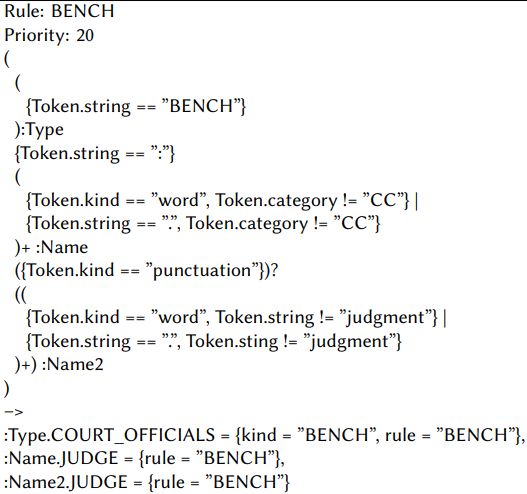
\includegraphics[width=80mm]{Screenshot from 2023-01-20 06-33-39.png}\\
    {\tiny {\color{red} BENCH}{\color{green}:}{\color{blue}Justice D. Y. Chandrachud}, {\color{magenta} Justice R. K. Krishna}}
\end{frame}

\begin{frame}[c]
    \centering 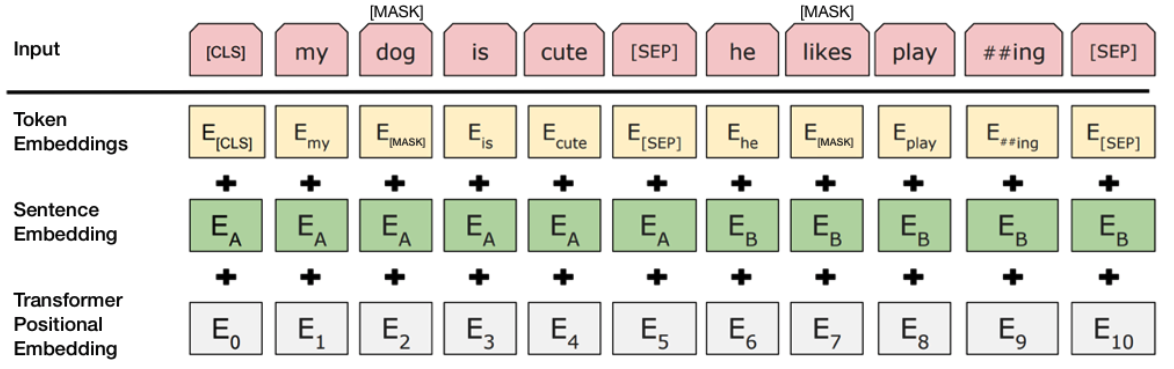
\includegraphics[width=100mm]{0_m_kXt3uqZH9e7H4w.png}\\
    \centering {\tiny Source: BERT (Devlin et. al., 2018)}
\end{frame}

\begin{frame}[c]
    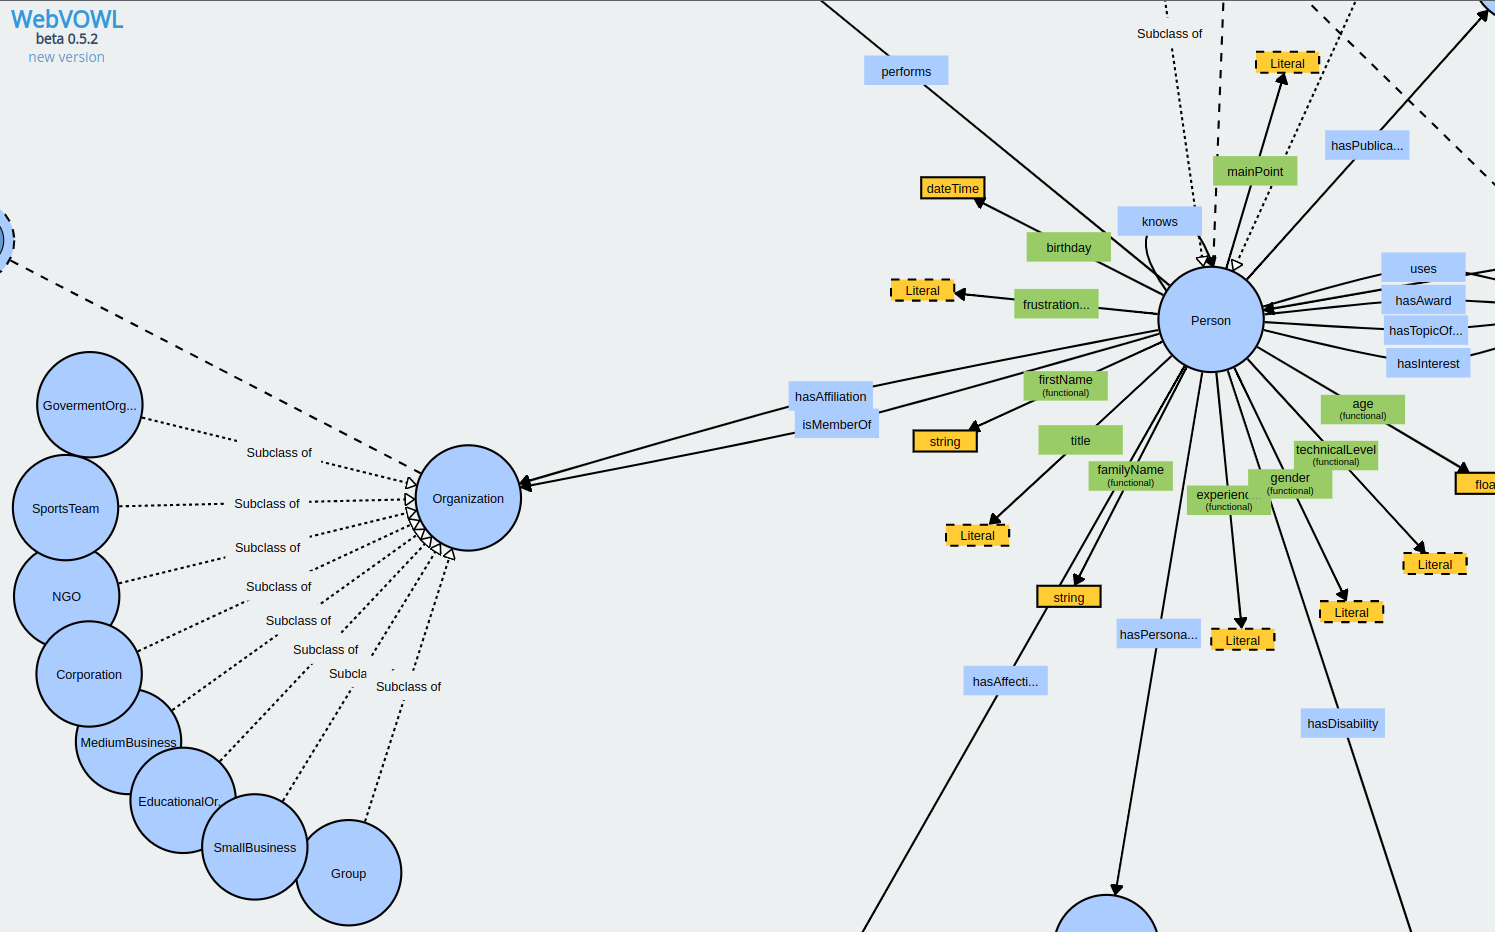
\includegraphics[width=120mm]{Screenshot from 2023-01-20 06-19-57.png}
    \centering {\tiny Source: PersonasOnto}
\end{frame}

\subsection{Question Understanding}
\begin{frame}
    \frametitle{Question Understanding}
    \begin{itemize}
    \small{\item Understanding natural language questions refers to the ability to break down a question into the requisite steps for computing its answer.
    \item Encode questions into low-dimensional vectors with contextual information?
    \item Calculate semantic similarity between questions and entities in KB?
    \item Detect and link entities in questions to those in KB and construct queries?}
    \end{itemize}
    \begin{block}{Question}
        \scriptsize{{\color{violet} What} drug is {\color{teal} prescribed for} treating {\color{red} fever}{\color{violet} ?}}
    \end{block}
    \begin{block}{Parsed Query}
        \tiny{<{\color{red} ?}, {\color{teal} prescribed for}, {\color{red} fever}>}
    \end{block}
    \begin{block}{Semantic Query}
        \tiny{<{\color{red} ?}, {\color{teal} https://www.wikidata.org/wiki/Property:P2176}, {\color{red} https://en.wikipedia.org/wiki/Fever}>}
    \end{block}
\end{frame}

\begin{frame}[c]
    \frametitle{How?}
    \begin{itemize}
        \item Use language model to convert natural language questions to queries.
        \item Use the correct pattern matching strategy - SPARQL.
        \item Slot-filling values from question to queries.
        \item Running the query and retrieving triples.\\
    \end{itemize}
    \begin{block}{SPARQL - Querying Language}
        \tiny Data:\\{\tiny <http://example.org/book/book1> <http://purl.org/dc/elements/1.1/title> "SPARQL Tutorial" .\\
        <http://example.org/book/book2> <http://purl.org/dc/elements/1.1/title> "Artificial Intelligence" .}\\~\\
        Query:\\
        {\tiny SELECT ?book ?title
WHERE
\{
  ?book <http://purl.org/dc/elements/1.1/title> ?title .
\}}\\~\\
        Result:\\
        {\tiny <http://example.org/book/book1>, "SPARQL Tutorial"\\
        <http://example.org/book/book2>, "Artificial Intelligence"}
    \end{block}
\end{frame}

\begin{frame}
    \frametitle{Question Understanding (contd.)}
    \begin{itemize}
    \small{\item Generate semantically similar queries?
    \item Rank templates matching question?}
    \end{itemize}
    \begin{block}{KB Inferencing}
        Given a question $Q$, match that with a template that is semantically similar and find a set of triples from the KG that are similar to the entities or relations in the question, find top $K$ triples that might answer the template.
    \end{block}
    
    \begin{block}{Example}
        \tiny Question: What are the different book titles that are available?\\~\\
        Query:\\
        {\tiny SELECT ?book ?title
WHERE
\{
  ?book <http://purl.org/dc/elements/1.1/title> ?title .
\}} (\~99\%)\\
{\tiny SELECT ?book ?title
WHERE
\{
  ?book <http://random.org/concept/movie-title> ?title .
\}} (\~1\%)\\~\\
        Result:\\
        {\tiny <http://example.org/book/book1>, "SPARQL Tutorial"\\
        <http://example.org/book/book2>, "Artificial Intelligence"}
    \end{block}
\end{frame}


\subsection{Inferencing Engine}
\begin{frame}
    \frametitle{Inferencing Engine}
    \begin{itemize}
    \small{\item KBQA Models learn Question Answering by using a QA corpus and a populated KB -- uncertainty, incompleteness and noise are inevitable
    \item Probabilistic Inferencing $\implies$ infer predicates from templates.
    \item Offline -- learn the mapping between templates and predicates.
    \item Online -- break questions down to simple questions, make use of probability distributions, calculate maximum likelihood.
    \item Entity distribution, template distribution, value (answer) distribution.
    \item Questions in actual interactions might be vague and unusual.
    \item Answer questions with entities/predicates matching the top confidence score.}
    \end{itemize}
    \begin{example}
    \footnotesize{\textbf{Template:} what is {\color{teal} treated} by {\color{red} \$medicine}?\\
    \textbf{Predicate:} {\color{teal} prescribed\_for} (maybe 90.5\%), {\color{teal} founder} (maybe 0.01\%)}
    \end{example}
\end{frame}

\section{System Overview}
\subsection{Use Case Diagram}
\begin{frame}[c]
    \frametitle{Use Case Diagram}
    \begin{figure}
        \centering
        \def\svgwidth{\columnwidth}
        \resizebox{0.55\textwidth}{!}{\input{usecase.pdf_tex}}
    \end{figure}
\end{frame}

\subsection{System Architecture}
\begin{frame}[c]
    \frametitle{System Architecture}
    \begin{figure}
        \centering
        \def\svgwidth{\columnwidth}
        \resizebox{1.0\textwidth}{!}{\input{arch.pdf_tex}}
    \end{figure}
\end{frame}

\section{}
\begin{frame}
    \frametitle{References}
    \nocite{*}
    \printbibliography     
\end{frame}

\section{}
\begin{frame}[c]
    \centering
    \Huge Thank You
\end{frame}

\end{document}